\documentclass{standalone}
\usepackage{unicode-math}
\setmainfont{TeX Gyre Pagella}
\setmathfont{TeX Gyre Pagella Math}

\usepackage{pgfplots}
\pgfplotsset{compat = 1.18}

\begin{document}
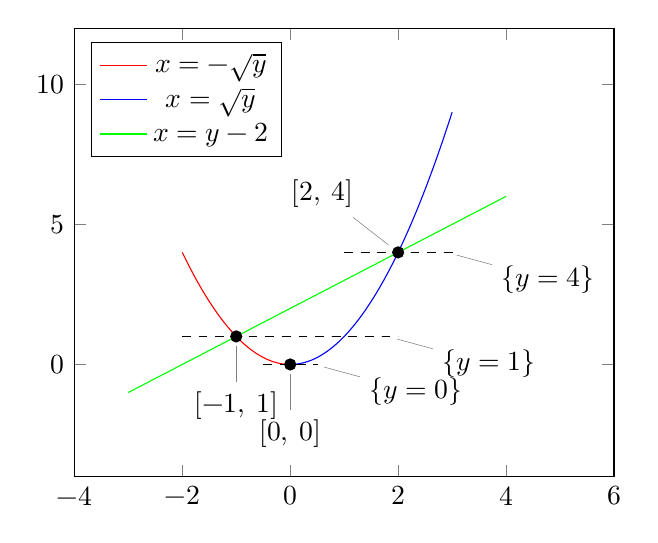
\begin{tikzpicture}
    \begin{axis}[
        legend style = {legend pos = north west},
        xmin = -4, xmax = 6,
        ymin = -4, ymax = 12
        ]
        \legend{\(x = -\sqrt{y}\), \(x = \sqrt{y}\), \(x = y - 2\)}
        \addplot [
            red,
            domain = -2:0,
            samples = 200,
        ]{x^2};

        \addplot [
            blue,
            domain = 0:3,
            samples = 200,
        ]{x^2};

        \addplot [
            green,
            domain = -3:4,
            samples = 200,
        ]{x+2};

        \addplot [
            black,
            dashed,
            domain = -2:2,
            samples = 200,
            pin edge = solid
        ]{1} node [pos = 0.95, pin = 355:{\(\left\{ y = 1 \right\}\)}] {};

        \addplot [
            black,
            dashed,
            domain = 1:3,
            samples = 200,
            pin edge = solid
        ]{4} node [pos = 0.95, pin = 355:{\(\left\{ y = 4 \right\}\)}] {};

        \addplot [
            black,
            dashed,
            domain = -0.5:0.5,
            samples = 200,
            pin edge = solid
        ]{0} node [pos = 0.95, pin = 355:{\(\left\{ y = 0 \right\}\)}] {};

        \addplot[
            only marks,
        ]
        coordinates{(-1, 1) (2, 4)}
        node [pos = 0, pin = 270:{\(\left[ -1,\: 1 \right]\)}] {}
        node [pos = 1, pin = 135:{\(\left[ 2,\: 4 \right]\)}] {};

        \addplot [
            only marks,
        ]
        coordinates{(0, 0)}
        node [pos = 0, pin = 270:{\(\left[ 0,\: 0 \right]\)}] {};
    \end{axis}
\end{tikzpicture}
\end{document}
